\documentclass[12pt,a4paper]{article}
\usepackage[utf8]{inputenc}
\usepackage[T1]{fontenc}
\usepackage{amsmath}
\usepackage{textcomp}

\usepackage{geometry}
\geometry{a4paper,left=25mm,right=25mm, top=2cm, bottom=2cm} 

\usepackage{graphicx} %fuer bilder

\usepackage{verbatim}




 \usepackage{mathptmx}
 \usepackage[scaled=.90]{helvet}
 \usepackage{courier}



\usepackage{listings}
\usepackage{color}
 
\definecolor{dkgreen}{rgb}{0,0.6,0}
\definecolor{gray}{rgb}{0.5,0.5,0.5}
\definecolor{mauve}{rgb}{0.58,0,0.82}

\pagestyle{empty}
\lstset{numbers=left,language=C++}
\lstset{showstringspaces=false,
basicstyle=\ttfamily\footnotesize,
breaklines=true,
tabsize=3,
commentstyle=\color{dkgreen},      % comment style
inputencoding={ansinew},
title=\lstname %zeigt titel der datei an
}

\usepackage{pdfpages} % fuer pdfs
\usepackage{hyperref} % fuer url


%keine einrückungen bei absatz
\parindent 0pt

\begin{document}
\title{Übung 01}
\author{Reinhard Penn, Bernhard Selymes}
\date{März 2015}

\normalsize

%Pfad zu c++ Dateien


%Beginn des Dokuments

\newcommand{\Uebung}{BFMVHDL}
\newcommand{\srcpath}{../../src}
\newcommand{\simpath}{../../sim}

%Angabe
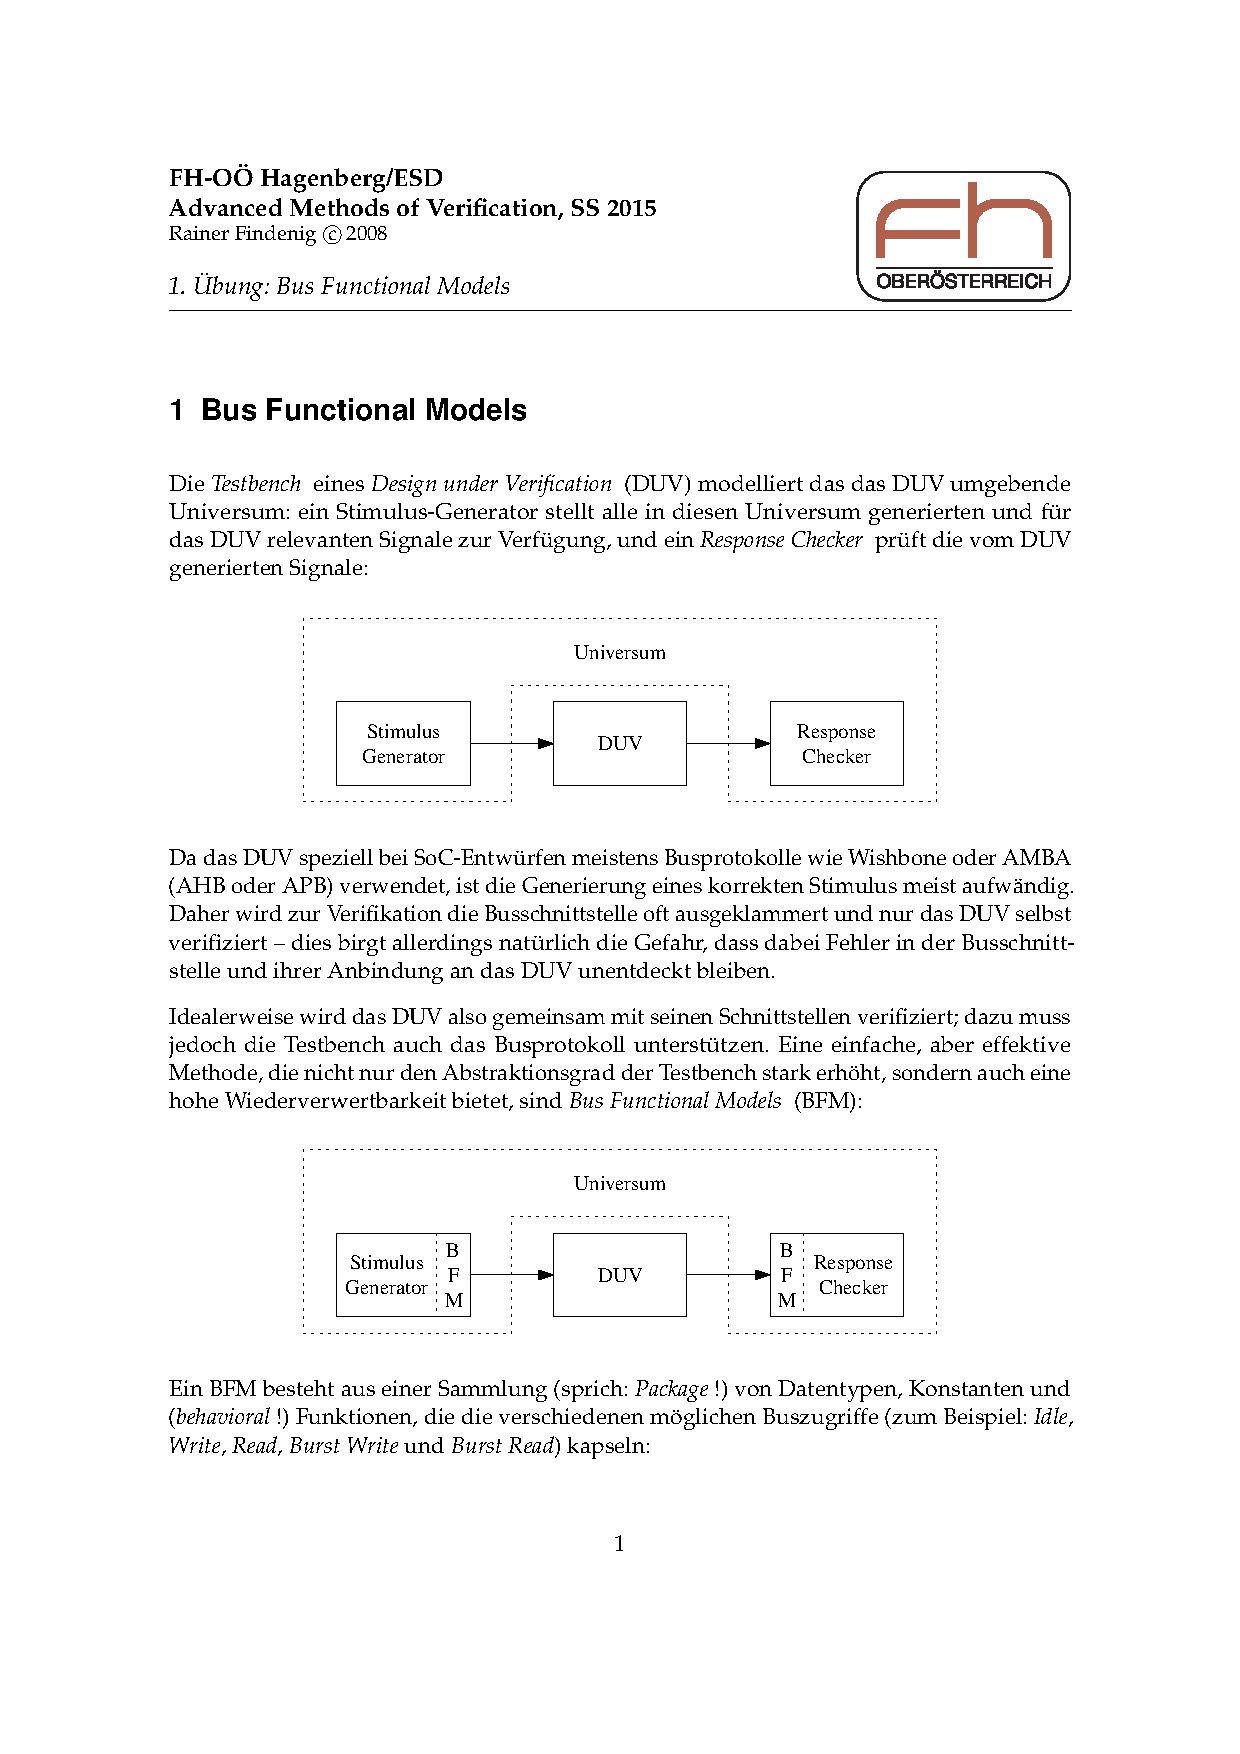
\includepdf[pages=-]{../Angabe.pdf}

\section{Beantwortung der Fragen}

\begin{itemize}
	\item Die VHDL-Anweisung \texttt{wait until} pausiert einen Prozess so lange bis sich eines der Signale im Statement ändert die gegebene Bedingung erfüllt ist. 
	Das heißt bei \texttt{wait until clk\_i = '1'} wird auf die steigende Flanke von \texttt{clk\_i} gewartet. Wenn \texttt{clk\_i} bereits \texttt{'1'} ist wird so lange gewartet bis wieder eine steigende Flanke kommt.
	\item Bei dieser VHDL-Anweisung wird so lange gewartet bis \texttt{ack\_i} während einer Änderung von \texttt{clk\_i '1'} ist.
	\item Das RAM könnte sonst nicht verbunden werden. In VHDL werden Signals verwendet um Parallelität zu modellieren.
\end{itemize}

Quelle: \url{http://www.ics.uci.edu/~jmoorkan/vhdlref}

\section{Testfälle}
Es wurden die unten aufgelisteten Funktionen der BFM getestet. Dazu wurde der gesamte Speicherbereich des RAM zweimal geschrieben und gelesen. Beim ersten Mal waren auf der Datenleitung alle geraden Bit 1 und ungeraden Bit 0. Beim zweiten Mal wurde der Wert invertiert. 
\\
Zusätzlich gibt es noch einen Idle Test der überprüft ob alle Signale auf 'Z' gesetzt sind und einen Test der zur Kontrolle fehlschlagen soll.
\\
Getestet wurde lokal am Rechner mit Questasim, da der Applicationserver bei beiden Gruppenmitgliedern nicht funktionierte.

\begin{itemize}
	\item SingleRead
	\item SingleWrite
	\item BlockRead
	\item BlockWrite
	\item Idle
\end{itemize}

\section{Source Code}

\lstinputlisting[language={VHDL}]{\srcpath/WishboneBFM-p.vhd}
\lstinputlisting[language={VHDL}]{\srcpath/WishboneBFM-tb.vhd}

\lstinputlisting[language={tcl}]{\simpath/Compile.do}
\lstinputlisting[language={tcl}]{\simpath/Sim.do}

\end{document}
